We continue with presenting two simple example methods that illustrate the motivation for using cached profiles.
The examples should provide the reader an indication of how and why cached profiles can be beneficial for the performance of a Java Virtual Machine.
We will omit any implementation details as they will be discussed in Chapter \ref{c:implementation} in detail.
\\\\
Ideally, being able to reuse the profiles from previous runs should result in two main advantages:
\begin{enumerate}
  \item \textbf{Lower start-up time of the JVM:} From having information about program execution, the compiler can avoid gathering profiles and compile methods earlier and directly at higher compilation levels.
  \item \textbf{Fewer Deoptimizations:} Since cache profiles are dumped at the end of a compilation, when using these profiles the compiler can already include all optimizations for all different method executions. The compiled code includes less uncommon traps and therefore fewer deoptimizations occur.
\end{enumerate}
\begin{figure}[ht!]
  \begin{center}
    \centering
    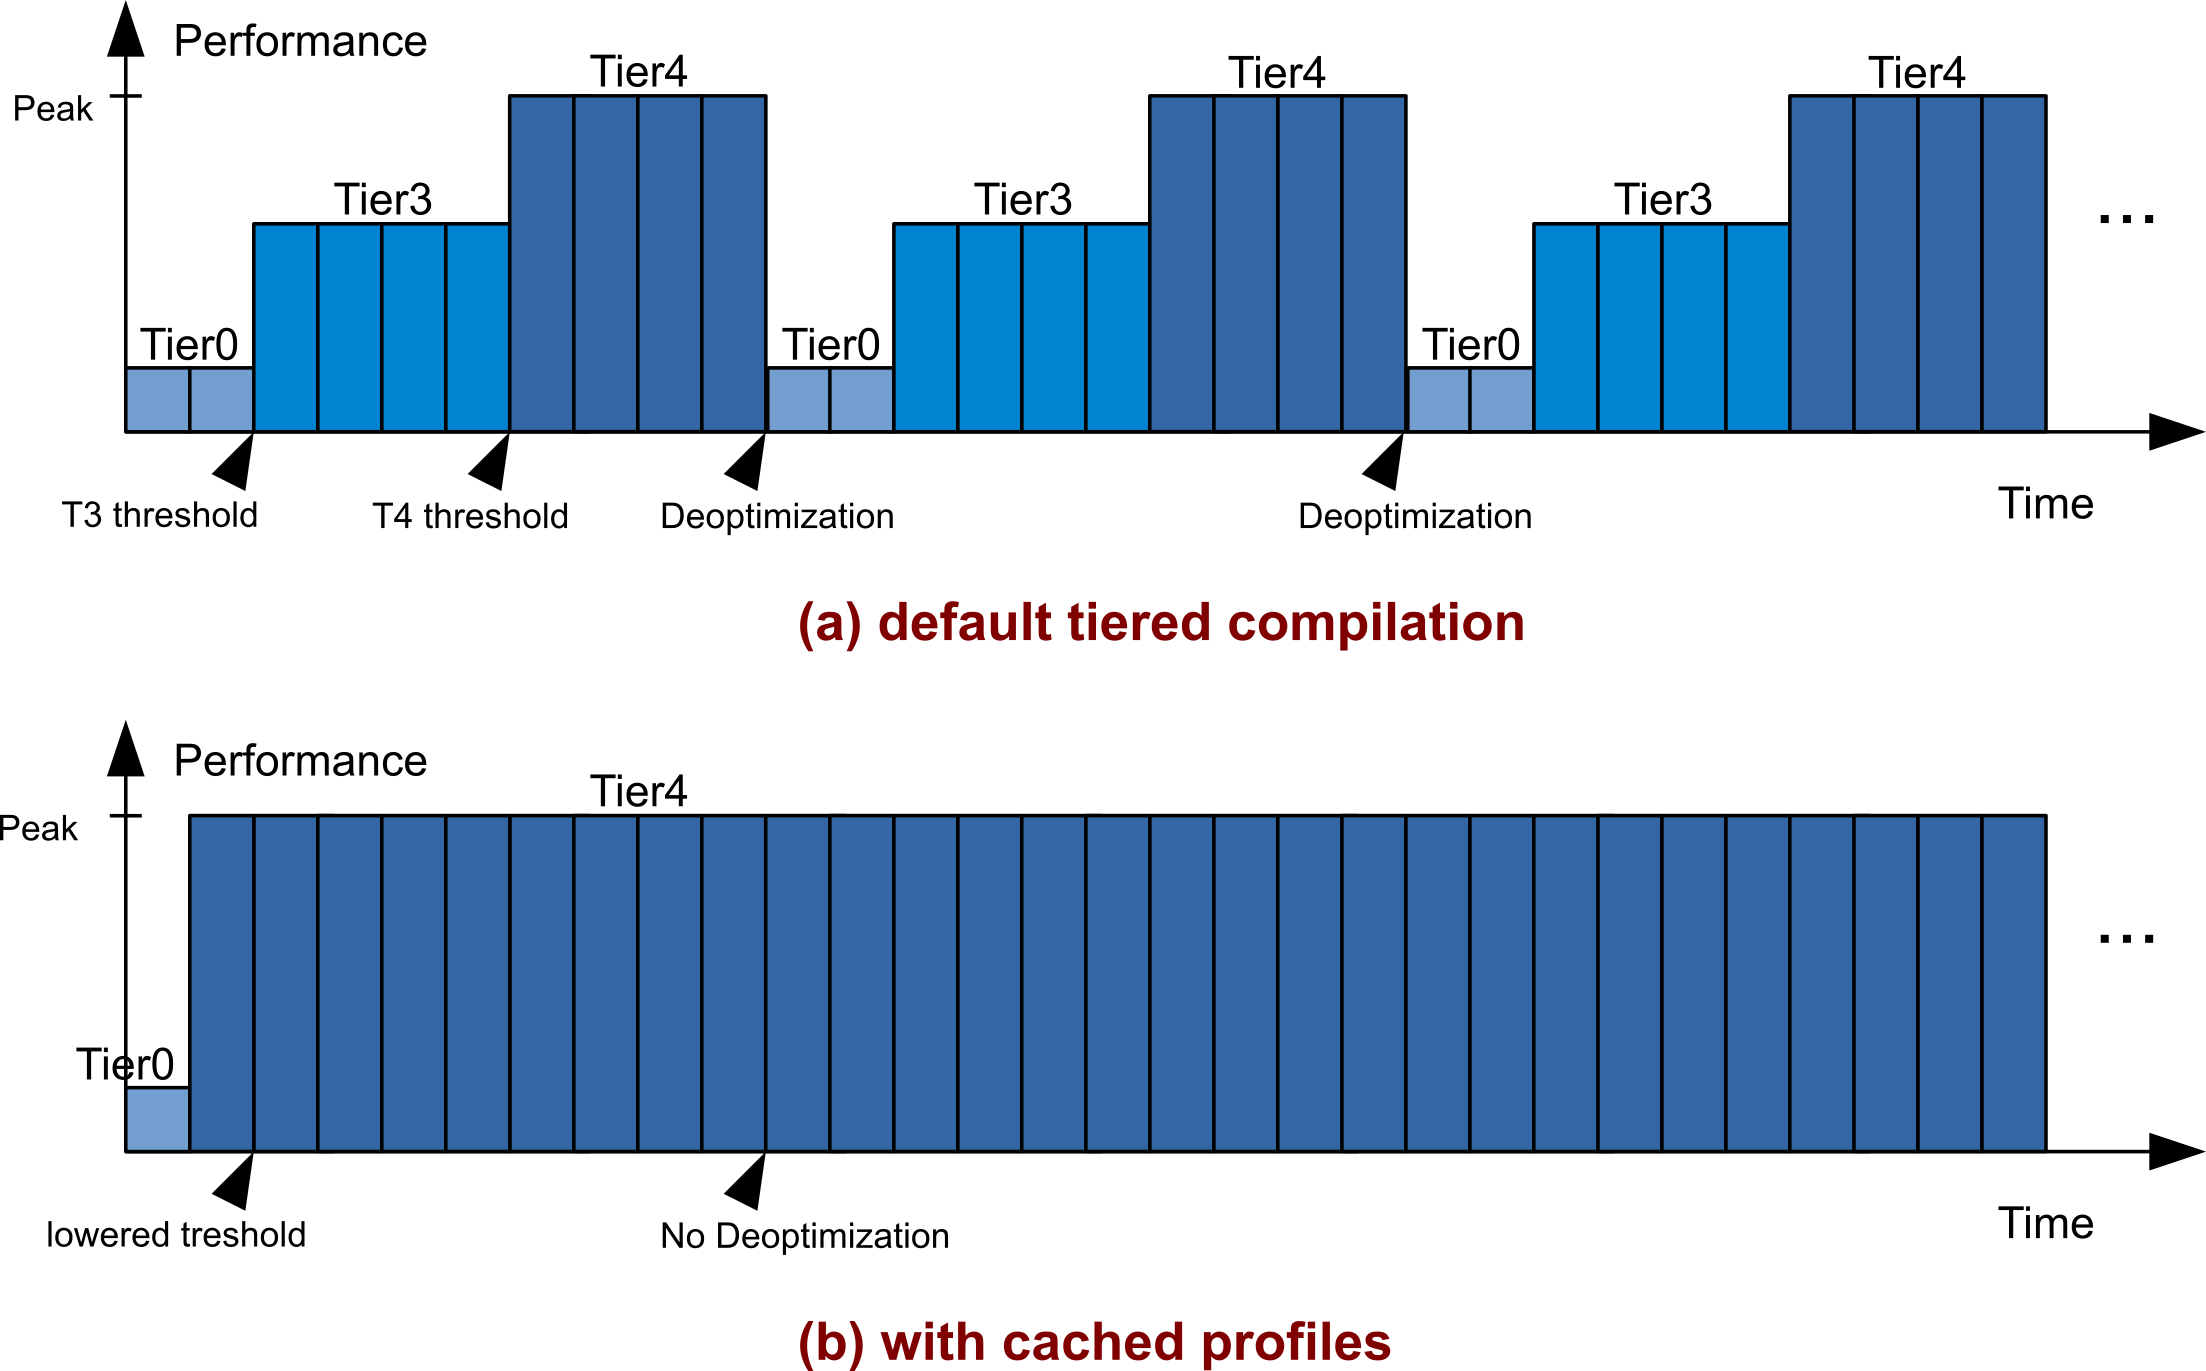
\includegraphics[width=0.8\textwidth]{figures/baseline_vs_usage_large.png}
    \caption{Schematic visualization of cached profile benefit}
    \label{f:baseline_vs_usage}
  \end{center}
\end{figure}
Figure \ref{f:baseline_vs_usage} gives a schematic visualization of the expected effect on the performance of a single method when using cached profiles compared to the current state without such a system and standard tiered compilation.
Each blue bar corresponds to an invocation of the method. Higher bars mean higher compilation levels and therefore higher performance. The x-axis represents time since the start of the JVM. The figure shows the ideal case and abstracts away many details and other possible cases. However, it provides a good visualization for the examples provided in this chapter. A more detailed performance analysis, also considering possible performance regressions is done in Chapter \ref{c:performance}.
\\\\
We are using my implementation described in Chapter \ref{c:implementation} in CachedProfileMode 0 (see \ref{s:mode0}) built into openJDK 1.9.0.
All measurements in this chapter are done on a Dual-Core machine running at 2 GHz with 8GB of RAM. To measure the method invocation time we use hprof \cite{hprof} and the average of 10 runs. The evaluation process has been automated using a couple of python scripts. The error bars show the 95\% confidence interval.
\section{Example 1: Benefit of early compilation}
\label{s:ex1}
For Example 1, on-stack replacement (OSR) has been disabled to keep the system simple and easy to understand.
\\
Example 1 is a simple class that invokes a method one hundred times. The method consists of a long running loop. The source code is shown in Listing \ref{l:nocompile}.
Since OSR is disabled and a compilation to level 3 is triggered after 200 invocations this method never leaves the interpreter. We call this run the \textit{baseline}.
To show the influence of cached profiles we use a compiler flag to lower the compile threshold explicitly and, using the functionality written for this thesis, tell HotSpot to cache the profile.
In a next execution we use these profiles and achieve a significantly lower time spend executing the cached method as one can see in Figure \ref{f:nocompile}.
This increase comes mainly from the fact that having a cached profile available allows the JVM to compile highly optimized code for hot methods earlier (at a lower threshold) since there is no need to gather the profiling information first.
\\\\
Since the example is rather simple neither the baseline nor the profile usage run trigger any deoptimizations. This makes sense because after the first invocation, all the code paths of the method have been taken already and are therefore known to the interpreter and saved in the profile.
\begin{lstlisting}[float,caption=Simple method that does not get compiled,label=l:nocompile,language=Java]
class NoCompile {
    public static void main() {
      double result = 0.0;
      for(int c = 0; c < 100; c++) {
        result = method1(result);
      }
    }
    public static double method1(double count) {
        for(int k = 0; k < 10000000; k++) {
            count = count + 50000;
        }
        return count;
   }
}
\end{lstlisting}
\begin{figure}[ht]
  \begin{center}
    \centering
    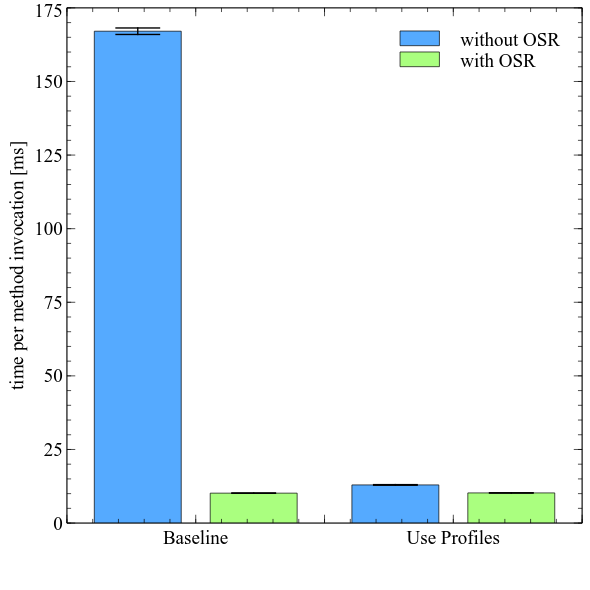
\includegraphics[width=0.5\textwidth]{figures/nocompile.png}
    \caption{NoCompile.method1 - per method invocation time}
    \label{f:nocompile}
  \end{center}
\end{figure}
\\\\
When OSR is enabled, the performance difference between using cached profiles and not using them vanishes.
That happens because HotSpot realizes the hotness of the method and the simplicity of the method allows the JIT compiler to produce optimized code already. The interpreted version is replaced on the stack by the compiled version during he first method invocation. 
The optimality of the compiled code is confirmed by the fact that no deoptimizations occur.
This example appears rather artificial since the same performance can be achieved with OSR already but nevertheless shows the influence of early compilation.
\section{Example 2: Benefit of fewer deoptimizations}
\label{s:ex2}
OSR is one of the core features of HotSpot to improve startup performance of a JVM and disabling that does not give us any practical results. We came up with a second more complex example sketched in Listing \ref{l:manydeopts}, that demonstrates the influence of cached profiles without disabling any HotSpot functionalities.
\\\\
The idea is to create a method that takes a different, long running branch on each of its method invocations. Each branch has been constructed in a way that it will trigger an OSR compilation. When compiling this method during its first iteration only the first branch will be included in the compiled code. The same will happen for each of the 100 method invocations. As one can see in Figure \ref{f:manydeopts} the baseline indeed averages at around 134 deoptimizations and a time per method invocation of 186 ms.
\\\\
Now we use a regular execution to dump the profiles and then use these profiles. So theoretically the profiles dumped after a full execution should include knowledge of all branches and therefore the compiled method using these profiles should not run into any deoptimizations. As one can see in Figure \ref{f:manydeopts} this is indeed the case. When using the cached profiles no more deoptimizations occur and because less time is spent profiling and compiling the methods the per method execution time is even significantly faster with averaging at 169 ms now.
\begin{lstlisting}[float,caption=Simple method that causes many deoptimizations,label=l:manydeopts,language=Java]
class ManyDeopts {
    public static void main() {
      double result = 0.0;
      for(int c = 0; c < 100; c++) {
        result = method1(result);
      }
    }
    public static long method1(long count) {
        for(int k = 0l; k < 10000000l; k++) {
            if (count < 10000000l) {
                count = count + 1;
            } else if (count < 30000000l) {
                count = count + 2;
                .
                .
                .
            } else if (count < 50500000000l) {
               count = count + 100;
            }
            count = count + 50000;
        }
        return count;
   }
}
\end{lstlisting}
\\\\\\\\\\\\
\begin{figure}[ht!]
  \begin{center}
    \centering
    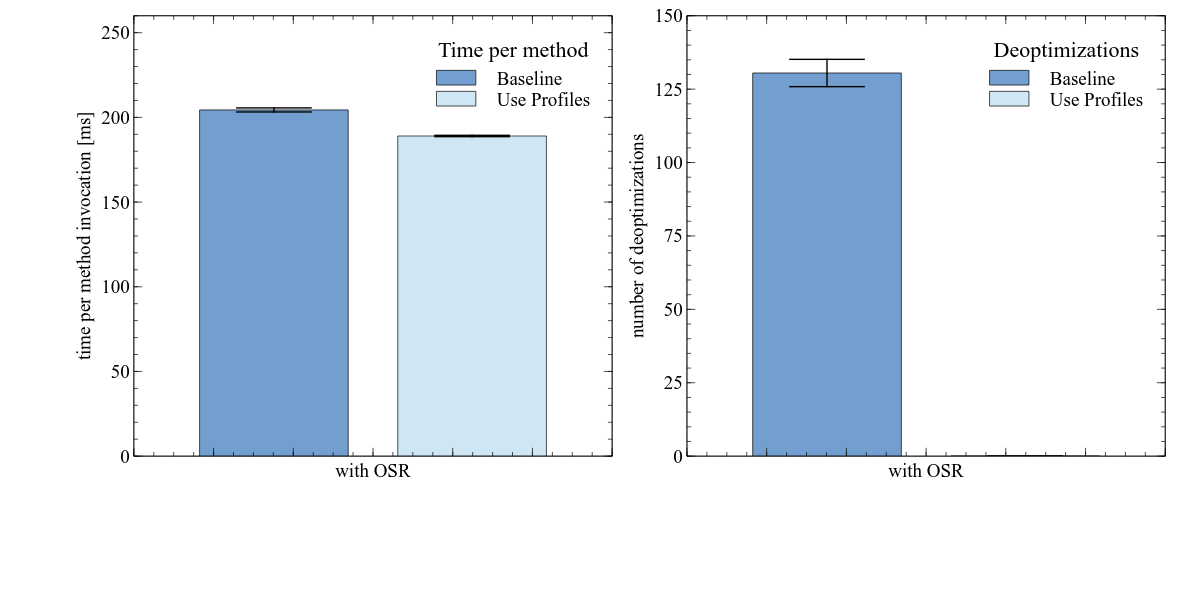
\includegraphics[width=0.9\textwidth]{figures/manydeopt.png}
    \caption{ManyDeopts.method1 - per method invocation time and deoptimization count}
    \label{f:manydeopts}
  \end{center}
\end{figure}
\\\\
\section{Similar systems}
\label{s:similarsystems}
In commercially available JVMs the idea of caching profiles is not new.
The JVM developed and sold by Azul Systems\textregistered\ called Zing\textregistered\ \cite{zing} already offers a similar functionality.
Zing\textregistered\ includes a feature set they call ReadyNow!\texttrademark\ \cite{readynow} which aims to increase startup performance of Java applications.
Their system has been designed with financial markets in mind and to overcome the issue of slow performance in the beginning and performance drops during execution.
\\\\
Azul Systems clients reported that their production code usually experiences a significant performance decrease as soon as the market goes live and the clients start trading.
The reasons are deoptimizations, that occur for example due to uncommon branch paths being taken or yet unused methods are invoked.
In the past Azul Systems' clients used techniques to warm up the JVM, for example doing fake trades prior to market opening. However this does not solve the problem sufficiently well, since the JVM optimizes for these fake trades and still runs into deoptimizations once actual trades happen, because the code includes methods or specific code snippets that differentiate between the fake and the real trades.
\\\\
ReadyNow!\texttrademark\ is a rich set of improvements how a JVM can overcome this issues. It includes attempts to reduce the number of deoptimizations in general and other not further specified optimizations.
As one of the core features Azul Systems\textregistered\ implemented the ability to log optimization statistics and decisions and reuse this logs in future runs. This is similar to the approach presented in this thesis. However they do not record the actual optimization but the learning and the reasons why certain optimizations happen. This gives them the ability to give feedback to the user of the JVM whether or not certain optimizations have been applied. They also provide APIs for developers to interact with the system and allow further fine-grained custom-designed optimizations.
\\\\
Unfortunately, Azul Systems does not provide any numbers about how their JVM actually improves performance when executing a software application or any analysis where the speedup originates from in detail.
